\documentclass[11pt,twoside,a4paper]{article}
\usepackage{authblk}  % For author affiliations with the basic article class
\usepackage{booktabs}  % For formal tables
\usepackage[margin=1in]{geometry}
\usepackage{graphicx}
\usepackage{hyperref}
\usepackage{mathtools}  % for \shortintertext{} and PairedDelimiter
\usepackage{xcolor}

\graphicspath{ {../figures/} }

\DeclarePairedDelimiter\p{(}{)}
\DeclarePairedDelimiter\brkt{[}{]}

\newcommand{\ariel}[1]{{\color{blue} Ariel: [{#1}]}}
\newcommand{\adam}[1]{{\color{green} Adam: [{#1}]}}
\newcommand{\strike}[1]{{\color{red} Strikeout: [{#1}]}}
\newcommand{\authoremail}[1]{\href{mailto:{#1}}{\textnormal{\texttt{{#1}}}}}

% Set the affiliation font and the affiliation separation
\renewcommand\Affilfont{\itshape\small}
\setlength{\affilsep}{1em}

\begin{document}

\title{AFQ-Insight}
\title{Multidimensional analysis and detection of informative features in diffusion MRI measurements of human white matter}
\date{\today}

\author[1]{Adam Richie-Halford\thanks{Corresponding author: \authoremail{richford@uw.edu}}}
\author[2]{Jason Yeatman}
\author[3]{Noah Simon}
\author[4]{Ariel Rokem}

\affil[1]{University of Washington Department of Physics, Seattle, WA 98105}
\affil[2]{University of Washington Department of Speech and Hearing Sciences, Seattle, WA 98105}
\affil[3]{University of Washington Department of Biostatistics, Seattle, WA 98105}
\affil[4]{University of Washington e{S}cience Institute, Seattle, WA 98105}

\section*{Abstract}

\adam{This is a copy of the abstract submitted for SfN 2018}
% Please keep the abstract below 300 words

The white matter contains long-range connections between different brain regions. Tractometry uses diffusion-weighted magnetic resonance imaging (dMRI) data to quantify tissue properties along the trajectories of these connections in the human brain in vivo\cite{yeatman2012tract}. In previous work, the results of tractometry were usually analyzed using mass univariate approaches: group comparisons or regression models computed separately for each point along every one of the tracts.  Alternatively, tissue properties such as fractional anisotropy (FA) and mean diffusivity (MD) were computed for a specific tract of interest based on an a priori hypothesis. In the present work, we developed a method based on the sparse group lasso\cite{simon2013sparse} that takes into account all of the tissue properties measured in all of the tracts, and selects informative features by enforcing sparsity, both at the level of individual tracts and tissue properties, but also across the entire set of tracts and all of the measured tissue properties. The sparsity penalties for each of these constraints is identified using a nested cross-validation scheme. Using data from a previous study that measured dMRI in patients with amyotrophic lateral sclerosis (ALS) and matched controls\cite{sarica2017corticospinal}, we demonstrate that this method is accurate, exceeding the previous results, that were based on a priori feature selection, in classifying patients and controls, with ~84\% accuracy, an area under the receiver operating characteristic curve of 0.93, and an average precision of 0.95. Moreover, our method automatically identifies as important for this classification the parts of the white matter known to be affected by ALS within the corticospinal tract. In a regression setting, data from another previous study\cite{yeatman2014lifespan} can be used to accurately predict ``brain age''. Thus, this multivariate analysis approach both (a) achieves high cross-validated accuracy for precision medicine applications of dMRI data and (b) identifies relevant features of brain anatomy to further our neuroscientific understanding of clinical disorders.


\maketitle
\tableofcontents

\section*{Introduction}

Diffusion-weighted Magnetic Resonance Imaging (dMRI) provides a unique
view into the physical properties of the connections that comprise
the brain white matter. While the measurements are usually conducted
with voxels at the millimeter scale, water molecules within each voxel
diffuse with characteristic lengths at the micrometer scale, providing
aggregate information about the physical structure of the white matter,
including the density of axons and distribution of fiber
orientations within each voxel \cite{wandell2016clarifying}. Even though
metrics derived from diffusion measurements are ambiguous in terms
of their underlying biological interpretation \cite{Jones2013-xv},
analyzing the variance in these properties has proven useful in
characterizing individual differences in cognitive function,
characterizing differences between populations and detecting brain
abnormalities associated with disease \cite{Thomason2011-qn}.

To relate the diffusion in each voxel to the macro-structure of
long-range connections between different brain regions, methods for
computational tract-tracing from diffusion MRI, or tractography, combine
the estimates of fiber orientations in each voxel to form streamlines
that traverse the volume of the white matter \cite{Conturo1999-je,
Mori2002-qi}. These methods have been under increased scrutiny and
several lines of investigation have raised critiques of their validity
\cite{Maier-Hein2017-vb, Thomas2014-ki}. On the other hand, there
have been efforts to shore up the inferences made with these methods
\cite{Pestilli2014NatMeth, Takemura2016-sh, Smith2013-nc, Smith2015-cx,
Smith2015-zt, Rheault2018-wk}. Importantly, though discovering novel
tracts requires extraordinary evidence, and delineating
the exact cortical termination of the streamlines in the gray matter
is still prone to error, there is little dispute that tractography
can accurately define the location of several major white matter
tracts that are known to exist within the core of the white matter
\cite{Maier-Hein2017-vb}.

Leveraging this fact, one of the most powerful methods currently
available to put macro- and micro-structure together is
\emph{tractometry}: assessment of the physical properties of the white
matter along specific tracts \cite{Bells2011-cf}. Though there are
several different available implementations of this overall idea,
the principles are similar \cite{yeatman2012tract, Yendiki2011-ay,
Wassermann2016-iv, ODonnell2009-uu}: tractometry begins by delineating
the parts of the white matter that belong to different major ``tracts''
(i.e. anatomical or functional groups of white matter fibers),
such as the corticospinal tract or arcuate fasciculus, assigning
tractography generated streamlines to ``bundles,'' which approximate
the anatomical tracts, and sampling biophysical properties (such as
fractional anisotropy or mean diffusivity) along the length of these
bundles. Whereas the identification of the anatomical correlates
of tractography-generated streamlines is an open problem, the
correspondence between tractometry's bundles and anatomical tracts is
well supported \cite{Catani2002-vu}. Tract-based diffusion metrics are
therefore appropriate degrees of freedom with which to understand the
white-matter correlates of cognitive function or disease.

In some previous tractometry-based studies, tissue properties along
the length of each tract were summarized by taking the mean along
each bundle, but there is a large body of evidence showing that there
is systematic variability along the trajectory of each bundle. This
justifies retaining the individual samples along the length of each
bundle \cite{yeatman2012tract, colby2012, ODonnell2009-uu}. While this
retains important information about each individual's white matter, it
also presents statistical challenges due to the dimensionality of the
data. Based on tractometry, researchers may choose to compare different
individuals to each other. This is usually done according to one of the
following approaches:

\begin{enumerate}

\item Mass univariate approaches: In this approach comparisons between
groups or across individuals are done independently at each node
of each tract, for each one of the diffusion metrics available at
that point. This approach is exhaustive, but statistical power is
compromised by a multiple comparison problem. Different approaches
can be taken to resolving this challenge. For example, Colby and
colleagues \cite{colby2012} used a non-parametric resmapling approach to
correct for family-wise error across the different possible comparisons
\cite{Nichols2002-zu, Nichols2003-yy}.

\item Region of interest(ROI)-based approaches: An alternative that
circumvents the multiple comparison problem is to select just a few
tracts to compare in each individual, or even focusing on particular
segments of these tracts based on \emph{a priori} hypotheses. This
approach is very powerful when the biological basis of the process
of interest is relatively well understood (for a recent example, see
\cite{huber2018rapid}).

\item ROI-based selection, followed by multivariate analysis: Here,
an ROI is selected based on \emph{a priori} knowledge, and all the
nodes or voxels in the ROI are used together to fit a model that can
predict differences between individuals. An example of that is the
``profilometry'' framework, in which different diffusion metrics
from a single tract are combined together to provide input to a
multivariate analysis of covariance, and linear discriminant analysis
\cite{dayan2016profilometry}.

\end{enumerate}

Generally speaking, analysis methods should balance predictive
accuracy with descriptive power \cite{Murdoch2019-ax, Breiman2001-uz}.
Accordingly, tractometry analysis should simultaneously capitalize on
all the data across all tracts to make the best possible prediction,
while also retaining and elucidating spatial information about the
locations that are most informative for a prediction. In the present
work, we developed a novel framework for analysis of tractometry that
simultaneously selects the features for analysis, and fits a model
to these features. We use a linear modeling approach, which aims to
predict phenotypical variance in a group of subjects, based on a linear
combination of the features estimated with tractometry.

Using this approach, we first need to deal with the large and
asymmetric dimensionality of the data: tractometry data usually has
many more features (i.e., number of measurements per individual) than
samples (number of subjects), which makes inferences from the data
about phenotypical differences between individuals ill-posed. This
regime is the target of several statistical learning techniques, and
is often solved by various forms of regularization. For example,
Tikhonov regularization shrinks the solution such that the sum of
squared contributions from the individual features are minimized
\cite{Hoerl2000-ij}. Another solution to the problem is provided by
the Lasso algorithm, which instead minimizes the sum of the absolute
values of contributions of each feature \cite{Tibshirani1996-qs}. This
tends to shrink to zero the contributions of many of the features,
providing results that are both accurate and interpretable. When
additional structure is available in the organization of the data,
regularization algorithms can take advantage of this structure. For
example, if the features lend themselves to a natural division into
different groups, the group lasso (GL) can be used to select groups
of features, rather than individual features \cite{Yuan2006-ky}.
The Sparse Group Lasso (SGL) elaborates on this idea by providing
control both of group sparsity, as well as overall sparsity of the
solutions \cite{simon2013sgl}. Because the features measured with
tractomery lend themselves to grouping based on the tracts from which
each measurement is taken, GL and SGL could provide a useful tool
for linear model fitting in problems of this form. Here we, first,
develop an implementation of SGL that is well suited to the analysis of
tractometry data and, second, demonstrate the power and flexibility of
this approach by applying it to both classification (disease diagnosis)
and continuous prediction (age) problems from previously published
studies \cite{sarica2017corticospinal, yeatman2014lifespan}.

\section*{Materials and methods}

\subsection*{Data}

Two different previously-published datasets were used here:

\begin{enumerate}

\item Diffusion MRI from a previous study of the corticospinal
tract (CST) in patients with amyotrophic lateral sclerosis
(ALS \cite{sarica2017corticospinal}), containing data from 24 ALS
patients and 24 demographically matched healthy controls. These data
were measured in a GE Discovery 750 3T MRI scanner at the Institute
of Bioimaging and Molecular Physiology in Catanzaro. Informed consent
was provided as approved by the Ethical Committee of the University
``Magna Graecia'' of Catanzaro. Voxel resolution was \num{2x2x2}
$\text{mm}^3$ and 27 non-colinear directions were measured with a
$b=1000$ $\frac{\text{sec}}{\text{mm}^2}$. Here, both motion correction
and eddy current correction were applied before modeling the diffusion
tensor in each voxel. We will refer to this dataset as ALS.

\item Diffusion MRI data from a previous study of properties of
the white matter across the lifespan \cite{yeatman2014lifespan},
containing dMRI data from 76 subjects with ages 6-50. These data were
measured in a GE Discovery 750 3T MRI scanner at the Stanford Center
for Cognitive and Neurobiological Imaging. The Stanford University
IRB approved the procedures of this study. Informed consent was
obtained from each adult participant, and assent for participation
was provided by parents/guardians for children. Voxel resolution was
\num{2x2x2}$\text{mm}^3$ with 96 non-colinear directions measured with a
$b=2000$ $\frac{\text{sec}}{\text{mm}^2}$ and 30 non-colinear directions
measured with a $b=1000$ $\frac{\text{sec}}{\text{mm}^2}$. Data was
preprocessed to correct for subject motion and the diffusion tensor
model \cite{basser1994mr} was fit in every voxel, using a robust fit
\cite{chang2005restore}. These data were acquired using a dual spin echo
sequence, in which there is sufficient time for eddy currents to subside
between the application of the gradients and the image acquisition, so
no eddy current correction was applied. We will refer to this dataset
as WH.

\end{enumerate}

Data from both of these studies was processed in a similar manner,
using the Matlab Automated Fiber Quantification toolbox (AFQ)
\cite{yeatman2012tract}: streamlines representing fascicles of white
matter tracts were generated using a determinstic tractography algorithm
that follows the prinicpal diffusion direction of the diffusion tensor
in each voxel (STT) \cite{basser2000vivo}. Major tracts were identified
using multiple criteria: streamlines are selected as candidates for
inclusion in a bundle of streamlines that represents a tract if they
pass through known inclusion ROIs and do not pass through exclusion
ROIs \cite{wakana2007reproducibility}. In addition, a probabilistic
atlas is used to exclude streamlines which are unlikely to be part of
a tract \cite{Hua2008-sh}. Each streamline is resampled to 100 nodes
and the robust mean at each location is calculated by estimating the 3D
covariance of the location of each node and excluding streamlines that
are more than 5 standard deviations from the mean location in any node.
Finally, a bundle profile of tissue properties in each bundle was created
by interpolating the value of MRI maps of these tissue properties to the
location of the nodes of the resampled streamlines designated to each
bundle. In each of 100 nodes, the values are summed across streamlines,
weighting the contribution of each streamline by the inverse of the
mahalnobis distance of the node from the average of that node across
streamlines. This means that streamlines that are more representative of
the tract contribute more to the bundle profile, relative to streamlines
that are on the edge of the tract.

This process creates bundle profiles, in which diffusion measures
are quantified and averaged along twenty major fiber tracts. Here,
we use only the mean diffusivity (MD) and the fractional anisotropy
(FA) of the diffusion tensor, but additional dMRI-based maps or maps
based on other quantitative MRI measurements can also be used. These
bundle profiles, along with the phenotypical data we wish to explain
or predict, form the input to the SGL algorithm. In a domain-agnostic
machine learning context, the phenotypical data comprise the target
variables while the bundle profiles form the feature or predictor
variables (See Fig~\ref{fig:group-structure}).

\subsection*{Sparse Group Lasso}

Before fitting a model to the data, imputation and standardization are
performed. Missing node values (e.g., in cases where AFQ designates a node as
not-a-number) are imputed via linear interpolation. Care is taken not to
interpolate across the boundaries between different bundles. Some diffusion
metrics will have naturally larger variance than others and may therefore
dominate the objective function and make the SGL estimator unable to learn from
the lower variance metrics. For example, fractional anisotropy (FA) is bounded
between zero and one and could be overwhelmed by an unscaled higher-variance
metric like the mean diffusivity (MD). To prevent this we remove each feature's
mean and scale it to unit variance (z-score) using the
\lstinline{StandardScaler} from scikit-learn \cite{scikit-learn}. Scaling is
performed separately within each cross-validation set's training or testing data
to prevent leakage of information between the testing and training
sets\cite{kaufman2012leakage}.

After scaling and imputation, the tractometry data and target
phenotypical data can be organized in a linear model:
\begin{equation}
    y = \mathbf{X} \beta + \epsilon,
    \label{eq:lm}
\end{equation}
where $y$ is the phenotype -- categorical, such as a clinical diagnosis,
or continuous numerical, such as the subject's age. The tractometry
data is represented in the feature matrix $\mathbf{X}$, with rows
corresponding to different subjects, and columns corresponding
to diffusion measures at different nodes within each bundle. The
relationship between tractometric features and the phenotypic target is
characterized by the coefficients in $\beta$. The error term, $\epsilon$
is an unobserved random variable that captures the error in the model.
We denote our prediction of the targer phenotype as $\hat{y}$ and the
coefficients that produce this prediction as $\hat{\beta}$, so that
\begin{equation}
    \hat{y} = \mathbf{X} \hat{\beta},
    \label{eq:lm-approx}
\end{equation}
without the error term, $\epsilon$. In general, the feature matrix
$\mathbf{X}$ has dimensions $S \times (B \times N \times M)$, where $S$
is the number of subjects, $B$ is the number of white matter bundles,
$N$ is the number of nodes in each bundle, and $M$ is the number of
diffusion metrics calculated at each node. Typically, $B = 20$, $N =
100$, and $2 \le M \le 8$, resulting in $\sim 4,000 - 16,000$ features.
Conversely, many dMRI studies have between a few dozen and a few
hundred subjects, yielding a feature matrix that is wide and short.
Even in cases where more than a thousand subjects are measured (e.g.,
in the Human Connectome Project, where 1,200 subjects were measured
\cite{VanEssen2012}), the problem is ill-posed: the high dimensionality
of this data requires regularization to avoid overfitting and generate
interpretable results.

Here, we propose that in addition to regularizing the coefficients
in $\hat{\beta}$, we can also capitalize on our knowledge of the
group structure of the bundle profile features in $\mathbf{X}$. The
bundle-metric combinations form a natural grouping. For example, we
expect that MD features within the left arcuate fasciculus will
co-vary across individuals. Likewise for FA values within the right
corticospinal tract (CST) and so on. This group structure is represented
in Fig~\ref{fig:group-structure}, which depicts the linear model
$\hat{y} = \mathbf{X} \hat{\beta}$. Thus, we seek a regularization
approach that will fit a linear model with anatomically-grouped
covariates, where we expect to observe both groupwise sparsity, where
the number of groups (bundle/metric combinations) with at least one
non-zero coefficients is small, as well as within-group sparsity, where
the number of non-zero coefficients within each non-zero group is small.
The sparse group lasso (SGL) is a penalized regression technique that
satisfies exactly these criteria\cite{simon2013sparse}. It solves for a
coefficient vector
$\hat{\beta}$ that satisfies
\begin{equation}
    \hat{\beta} = \min_\beta \frac{1}{2}
    ||y - \displaystyle \sum_{\ell = 1}^{G}
    \mathbf{X}^{(\ell)} \beta^{(\ell)}||_2^2
    + \lambda_1 \displaystyle \sum_{\ell = 1}^{G}
    \sqrt{p_\ell} ||\beta^{(\ell)}||_2
    + \lambda_2 ||\beta||_1,
    \label{eq:sgl}
\end{equation}
where $G$ is the number of groups $\mathbf{X}^{(\ell)}$ is the submatrix
of $\mathbf{X}$ corresponding to group $\ell$, $\beta^{(\ell)}$ is
the coefficient vector for group $\ell$ and $p_\ell$ is the length of
$\beta^{(\ell)}$. In the tractomtetry setting, $G = T \times M$ and
$\forall \ell: p_\ell = 100$. The first term is the mean square error
loss, $L_{\text{mse}}$, as in the standard linear regression framework.
The second and third terms encourage groupwise sparsity and overall
sparsity, respectively. If $\lambda_1 = 0$ and $\lambda_2 = 1$, the
SGL reduces to the traditional lasso\cite{tibshirani1996regression}.
Conversely, if $\lambda_1 = 1$ and $\lambda_2 = 0$, the SGL reduces to
the group lasso\cite{yuan2006model}.

\begin{figure}[!h]
    \centering
    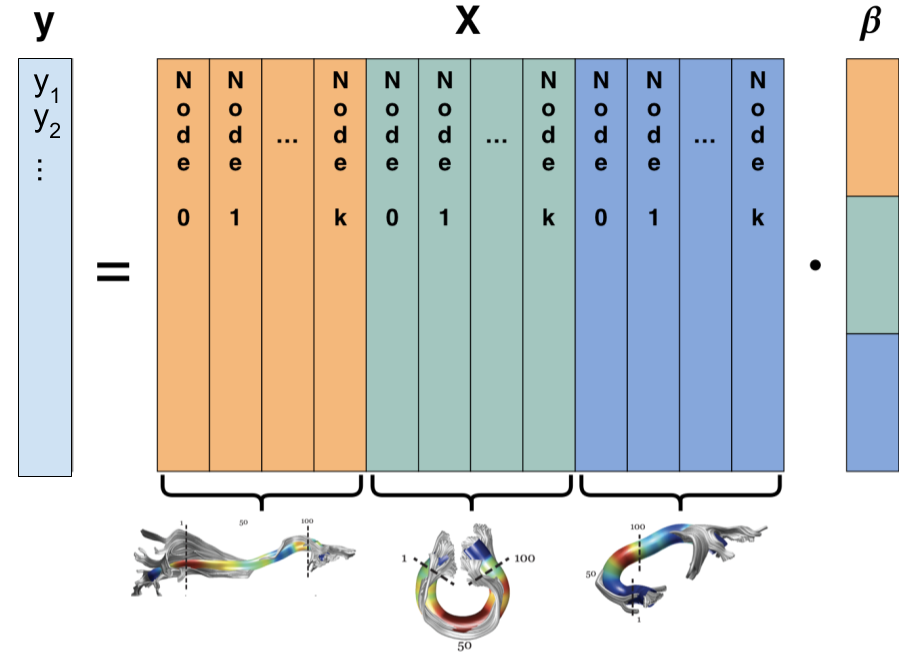
\includegraphics[width=0.65\textwidth]{dMRI_group_structure.png}
    \caption{{\bf dMRI group structure.}
        The phenotypical target data and tractometric features can
        be organized into a linear model, $\hat{y} = \mathbf{X}
        \hat{\beta}$. The feature matrix $\mathbf{X}$ is color-coded
        to reveal a natural group structure: the left (orange) group
        contains $k$ features from the inferior fronto-occipital
        fascicle (IFOF), the middle (green) group contains $k$ features
        from the corpus callosum, and the right (blue) group
        contains $k$ features from the uncinate. The coefficients in
        $\hat{\beta}$ follow the same natural grouping. Fascicle image
        reproduced with permission from Ref~\cite{yeatman2012tract}
        Figure 1.
    }
    \label{fig:group-structure}
\end{figure}


\subsubsection*{Incorporating transformations on $y$}

Often, the target variable $y$ is not in the domain in which the linear
model can be best fit to it. Equation \eqref{eq:lm-approx} can be slightly
modified as:
\begin{equation}
    \hat{y} = f^-1(\mathbf{X} \hat{\beta}),
    \label{eq:lm-transform}
\end{equation}
where the transformation function $f^{-1}$ characterizes the transform
applied to the data before fitting the linear coefficients. For example,
an often-used transform is the logarithmic transform:
\begin{equation}
    f(\hat{y}) = \log_n(\hat{y})
    \label{eq:log-nonlinearity}
\end{equation}
In this case, the model is parametrized by one additional fit parameter,
$n$.

\subsubsection*{Classification of categorical $y$}
When the phenotypical target variable is categorical, as in the case of
explaining or predicting the presence of a clinical diagnosis, the SGL is
readily adapted to logistic regression, where the probability of a target
variable belonging to an arbitrary defined ``true'' class is the logistic
function of the result of the linear model,
\begin{equation}
    p(\hat{y} = 1) = \frac{1}{1 + \exp(\mathbf{X} \hat{\beta})},
    \label{eq:logit}
\end{equation}
or equivalently, the mean squared error loss function in Eq~\eqref{eq:sgl} is
replaced with the cross-entropy loss, which for binary classification is the
negative log likelihood of the SGL classifier giving the ``true'' label:
\begin{equation}
    L_{\text{mse}} \rightarrow L_{\log} =
    -\left(y \log(p) + (1 - y) \log(1 - p)\right).
    \label{eq:logloss}
\end{equation}

\subsection*{Implementation, cross-validation and metaparameter optimization}

For given values of $\lambda_1$ and $\lambda_2$, the cost function in Eq~\eqref{eq:sgl} can be optimized using proximal gradient descent methods
\cite{parikh2014proximal} here implemented as a custom proximal operator that is
then optimized using the C-OPT library\cite{copt}. This supplies an estimate of
the optimal $\hat{\beta}$ given a particular set of values for the
meta-parameters $\lambda_1$ and $\lambda_2$.

To objectively evaluate the model and guard against over-fitting,
we used a nested cross-validation scheme, depicted in
Fig~\ref{fig:cross-val} for the categorical classification case.
The subjects (i.e. rows of the feature matrix $\mathbf{X}$ in
Fig~\ref{fig:group-structure} and Eq~\eqref{eq:lm}) are shuffled and
then decomposed into $k$ batches, hereafter referred to as folds. For
the ALS dataset we used $k=10$ and for the WH dataset $k=5$. For each
unique fold, we hold that fold out as the test\textsubscript{outer} set
and let the remaining data comprise the train\textsubscript{outer} set,
with the subscript indicating the depth of the nested decomposition.
We further decompose each train\textsubscript{outer} set into three
folds, and again for each unique fold, we hold out that fold as the
test\textsubscript{inner} set and let the remaining data comprise the
train\textsubscript{inner} set. At level-1 of the decomposition, we fit
an SGL model using fixed regularization meta-parameters $\lambda_1$
and $\lambda_2$, training the model using train\textsubscript{inner}
and evaluating the fit on test\textsubscript{inner}. We find
the optimal values for $\lambda_1$ and $\lambda_2$ using
hyperoptimization, implemented using the hyperopt library's \verb|fmin|
function\cite{Bergstra_2015} with a tree of Parzen estimators search
algorithm\cite{bergstra2011algorithms}. For continuous numerical $y$,
\verb|fmin| searches for meta-parameter values that minimize the median
absolute error. This can also be done minimizing the root of the mean
squared error (RMSE) or to maximizing the coefficient of determination
($R^2$). For binary categorical $y$ \verb|fmin| seeks to maximize the
classification accuracy. This can also be done maximizing the area
under the receiver operating curve (ROC AUC) or the average precision.
Using hyperoptimization, we find optimal regularization parameters and
$\hat{\beta}$ for each train\textsubscript{outer} set and then use those
to predict values for data in test\textsubscript{outer}. Thus each
subject in the dataset has a predicted phenotype derived from a model
that never saw its particular subject's data.

The above procedure describes $k$-fold cross validation. In fact, we use
repeated $k$-fold cross validation on the outer level of the decomposition, so
that the input data is decomposed into $k$ folds, three times. Thus, each
subject has three predicted phenotypes. We then take the mean predicted value to
summarize the performance of the model. In the classification case, the
shuffling into folds is stratified such that each fold has a population that
preserves the percentage of each class found in the larger input data.

\begin{figure}[!h]
    \centering
    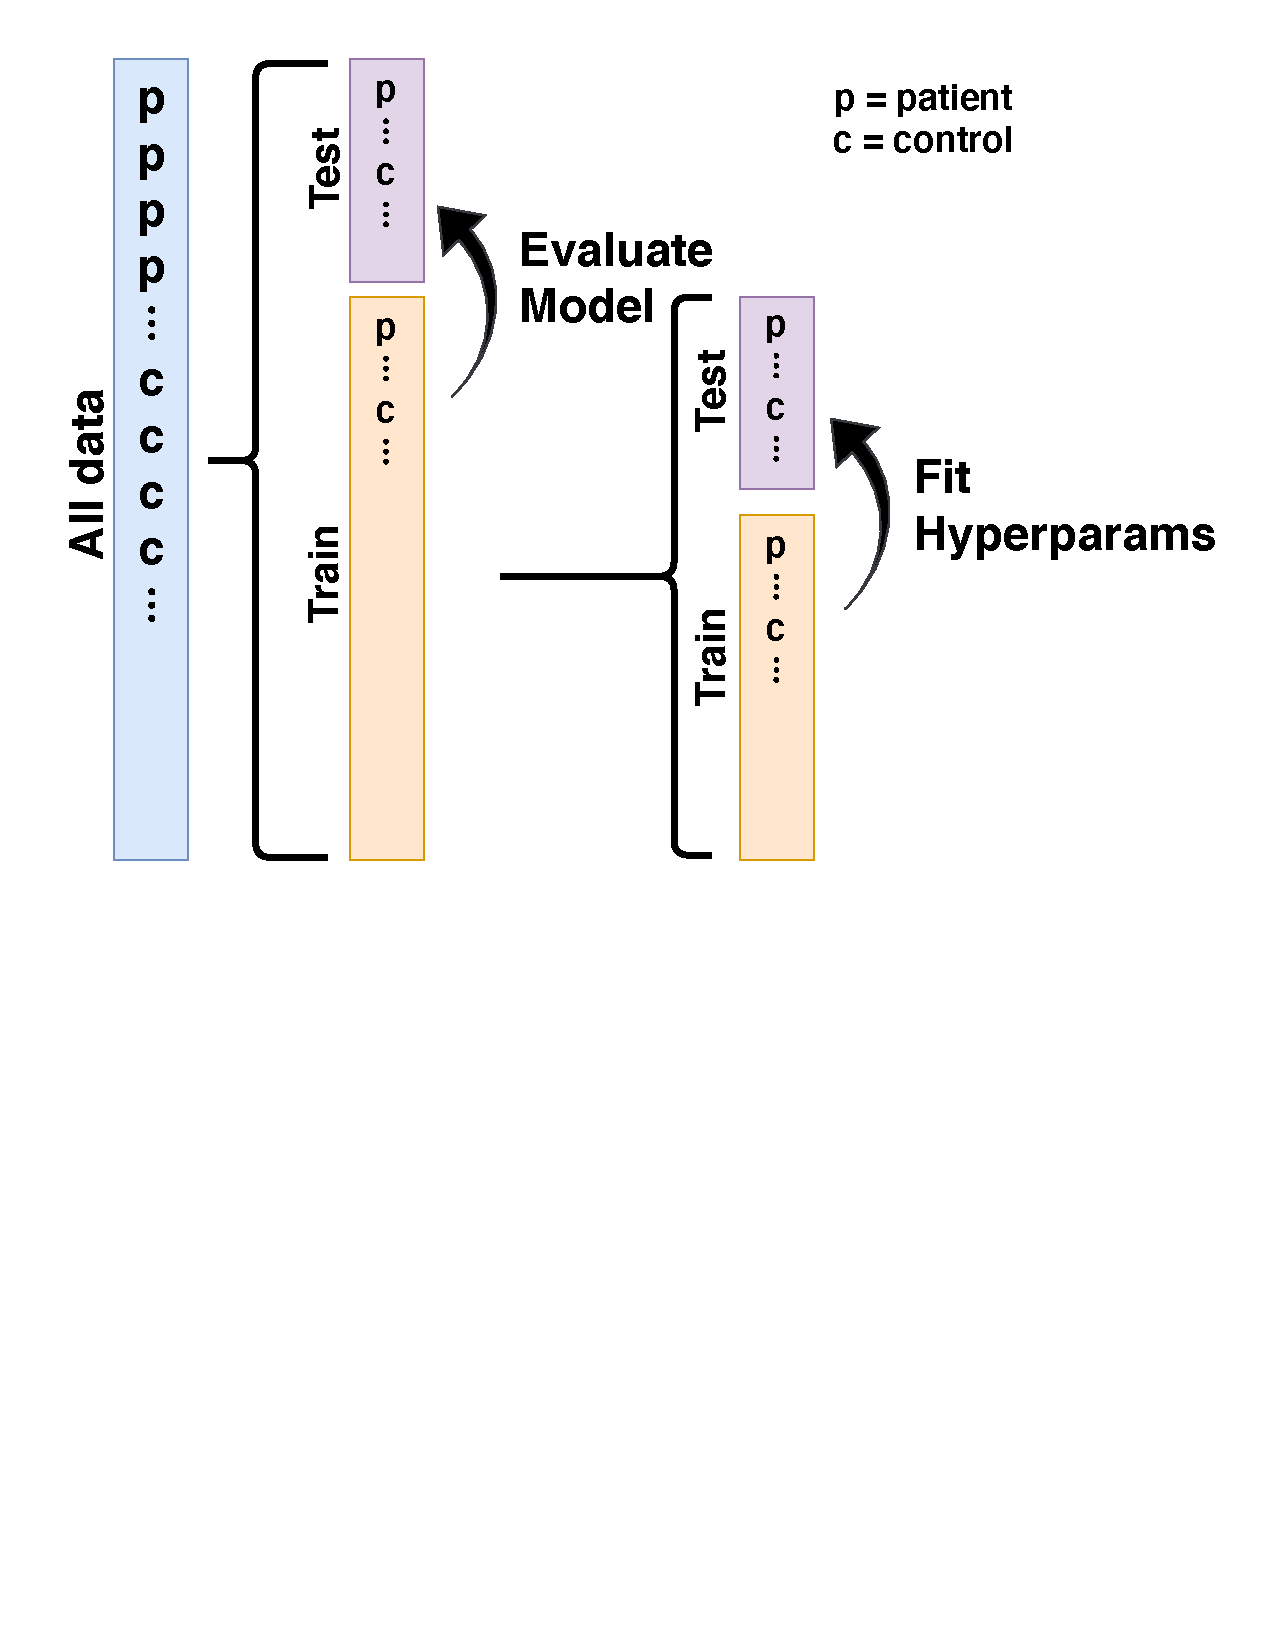
\includegraphics[width=0.55\textwidth]{nested-cross-validation.pdf}
    \caption{{\bf Nested $k$-fold cross-validation scheme.}
        We evaluate model quality using a nested $k$-fold cross
        validation scheme. At level-0, the input data is decomposed
        three times into $k$ shuffled groups and optimal hyperparameters
        are found for the level-0 training set. Optimization of these
        hyperparameters requires the use of the hyperopt library and
        many repeated evaluations of an SGL model over a search space
        of possible regularization parameters. These evaluations take
        place at level-1 of the decomposition, where the level-0 training
        set is further decomposed into three shuffled groups.
        For the ALS data, $k=10$. For the WH data, $k=5$.
    }
    \label{fig:cross-val}
\end{figure}

\subsection*{Software implementation}

The full software implementation of the SGL approach presented here is available
in a Python software package called AFQ-Insight, which is developed publicly in
\url{https://github.com/richford/afq-insight}. The version of the code used to
produce the results herein is also available in \ariel{Need to add Zenodo DOI}.
AFQ-Insight reads the target and feature data that has been processed by AFQ
from comma separated value (CSV) files conforming to the AFQ-Browser data
format\cite{yeatman2018browser} and represents them internally as
\lstinline{DataFrame} objects from the pandas Python
library\cite{mckinney2010data}. The software provides different options for
imputing missing data in the feature matrix. Missing interior nodes are imputed
using linear interpolation. For missing exterior nodes, the user may choose
between linear extrapolation and constant forward(back)-fill. Imputation uses
only values from adjacent nodes in the same white matter bundle in the same
subject so there is no danger of data leakage from other subjects. It uses the
scikit-learn\cite{scikit-learn} library to decompose input data into separate
test and train datasets, to scale each feature to have zero mean and
unit variance, and to evaluate each fit in the hyperparameter search using
appropriate classification and regression metrics such as accuracy, area
under the receiver operating curve (AUC ROC), and coefficient of determination
($R^2$). For each set of hyperparameters, we solve the SGL using a custom
proximal operator supplied to the C-OPT library\cite{copt}. Appropriate
hyperparameters are found using the hyperopt library\cite{Bergstra_2015}.

\section*{Results and discussion}

We developed a method for analyzing dMRI tractometry data with SGL. We
demonstrate the use of this method on two previously published datasets in both
a classification setting and a regression setting.

\subsection*{SGL accurately detects ALS in tractometry data in a classification setting}

Using data from a previous study of the corticospinal tract (CST) profile and
ALS\cite{sarica2017corticospinal}, we tested the performance of SGL in a
classification setting. The previous study predicted ALS status with a mean
accuracy of 80\% using a random forest algorithm based on a priori selection of
features within the corticospinal tract. SGL delivers competitive predictive
performance (mean 93\% $\pm$ 2\% accuracy, 0.978 $\pm$ 0.006 ROC AUC) without
the need for a priori feature engineering. The results of the classification
prediction are shown in Figure \ref{fig:class-results} with ``ground-truth'' ALS
status separated into columns, and predicted ALS status encoded by color. In
addition to this classification performance, SGL also identifies the white
matter tracts most important for ALS classification. The relative importance of
white matter features is captured in the $\beta$ coefficients from
Eq~\eqref{eq:sgl}. Figure \ref{fig:class-profiles} depicts these coefficients along
the right CST, plotted over the FA values for the control and ALS subject
groups. We find that SGL selects FA metrics in the corticospinal tract and
particularly in the right corticospinal tract as most important to ALS
classification, confirming previous findings\cite{van2011upper,
toosy2003diffusion, sarica2014tractography, sage2007quantitative,
sage2009quantitative, karlsborg2004corticospinal, ellis1999diffusion,
cosottini2005diffusion, ciccarelli2009investigation, abe2010voxel} and
identifying the portions of the brain that were selected \emph{a priori} in the
previous study from which we collected our data\cite{sarica2017corticospinal}.

Analyzing the ways in which the model mislabels individuals may also provide
insight. We found that mislabelled subjects are outliers relative to their group
with respect to diffusion features of the CST. Figure \ref{fig:class-errors}
depicts the group FA values along with FA values of mislabelled subjects, two
false negatives and one false-positive. The false negative classifications have
high FA in one of the two sections of the CST where $||\hat{\beta}|| > 0$ in
Figure \ref{fig:class-profiles}. The false positive subject has an FA that
oscillates between the two group means. Thus, the SGL method fails
comprehensibly.

\begin{figure}[h]
    \centering
    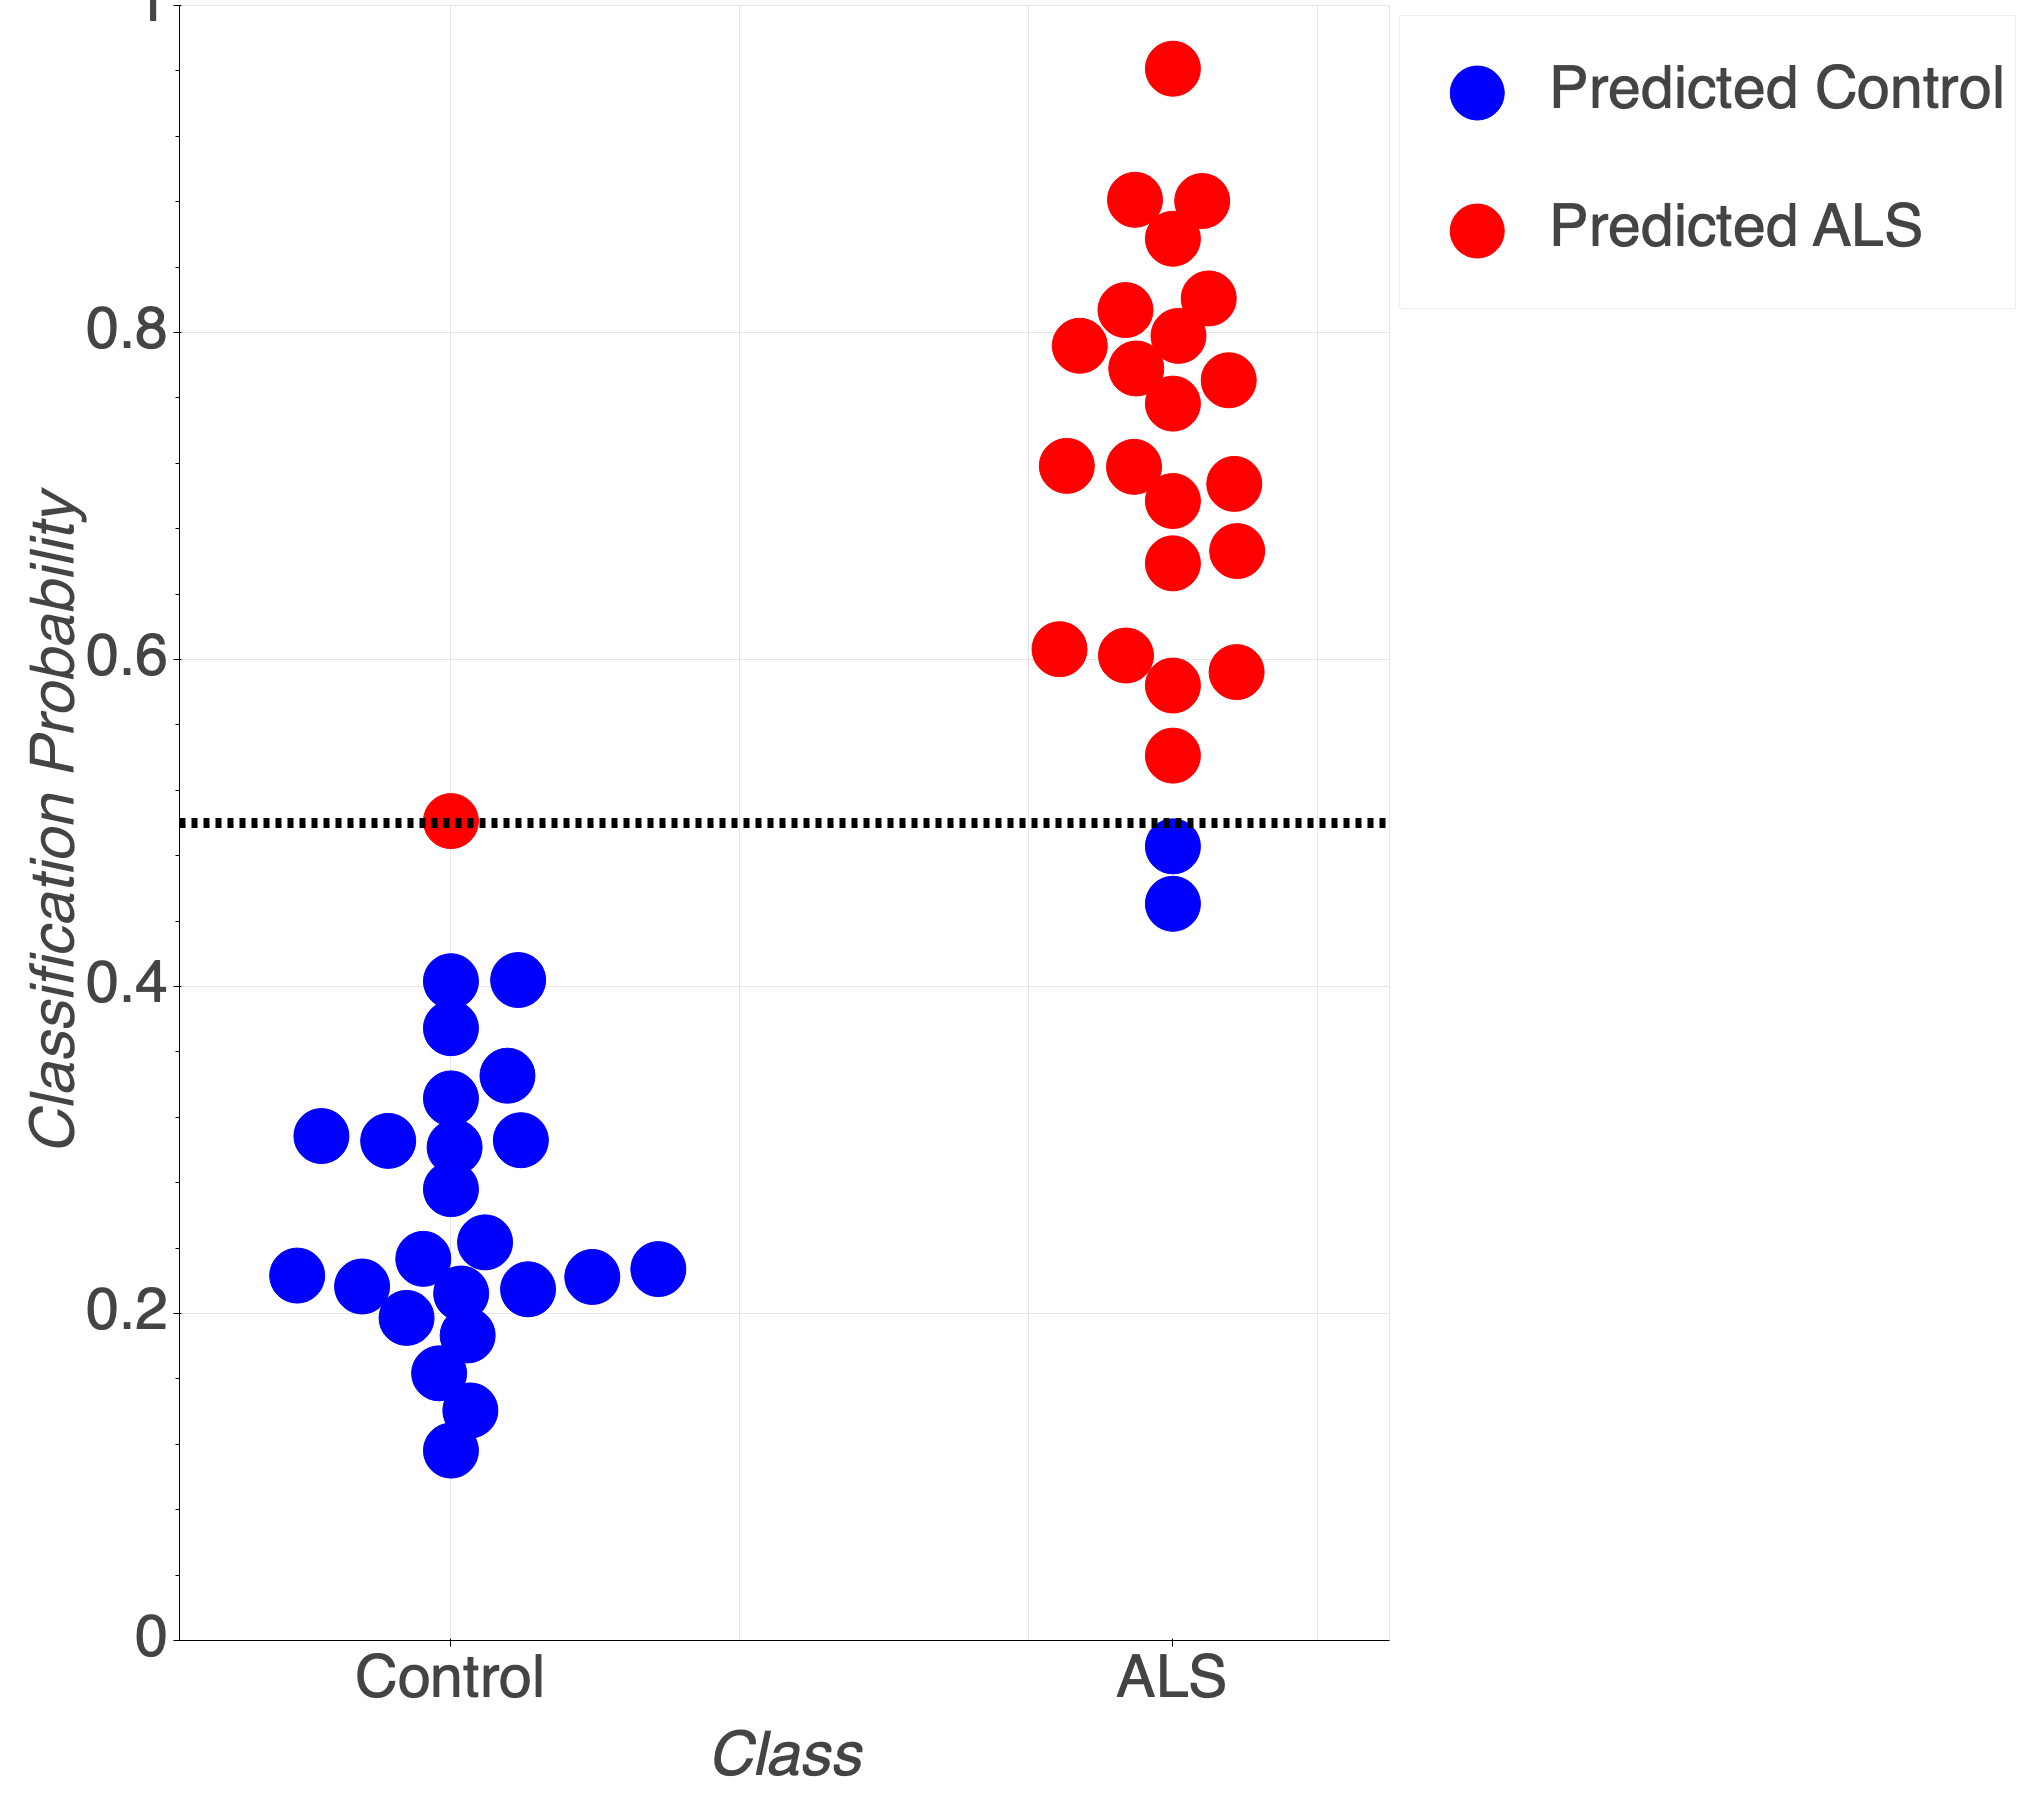
\includegraphics[width=0.45\textwidth]{classification_probs.png}
    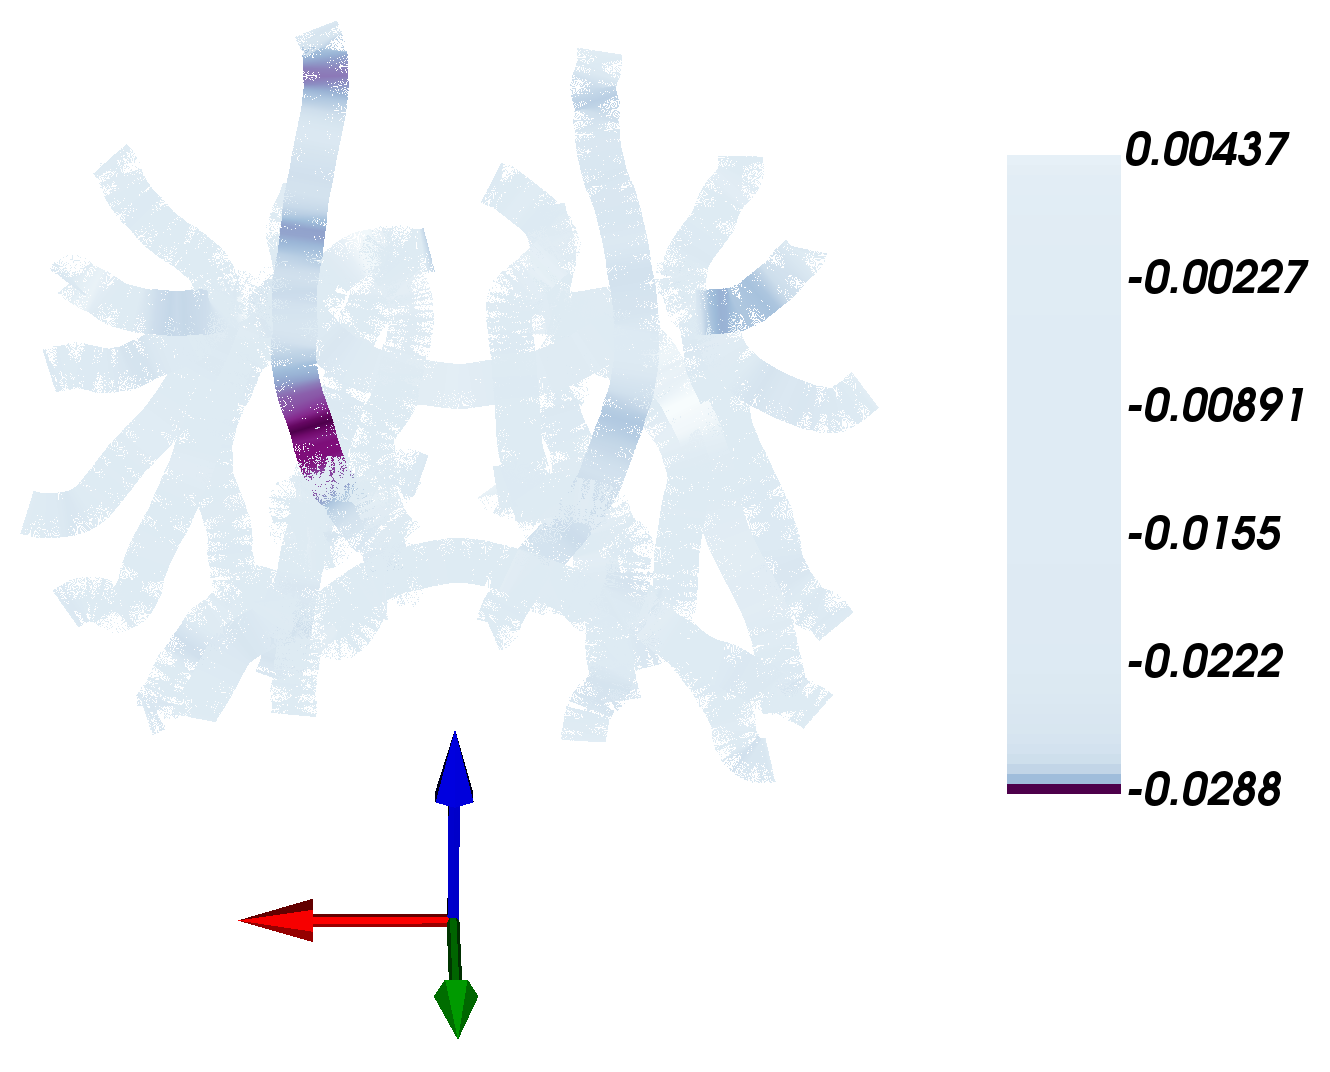
\includegraphics[width=0.45\textwidth]{classification_beta_bupu.png}

    \caption{{\bf SGL accurately predicts ALS.}
        Left: Classification probabilities for each subject's ALS diagnosis.
        Controls are on the left while patients are on the right. Predicted
        controls are in blue and predicted patients are in red. Thus, false
        positive are represented as red dots on the left, while false negatives
        are represented as blue dots on the right. The SGL algorithm achieves
        93\% $\pm$ 2\% accuracy,with 0.978 $\pm$ 0.006 ROC AUC. Right: SGL
        coefficients are presented on a skeleton of the major tracts. The brain
        is oriented with the right hemisphere to our left and anterior out of
        the page. As expected large negative coefficients are in the FA of the
        CST (and particularly in the right hemisphere, here to the left)}
    \label{fig:class-results}
\end{figure}

\begin{figure}[h]
    \centering
    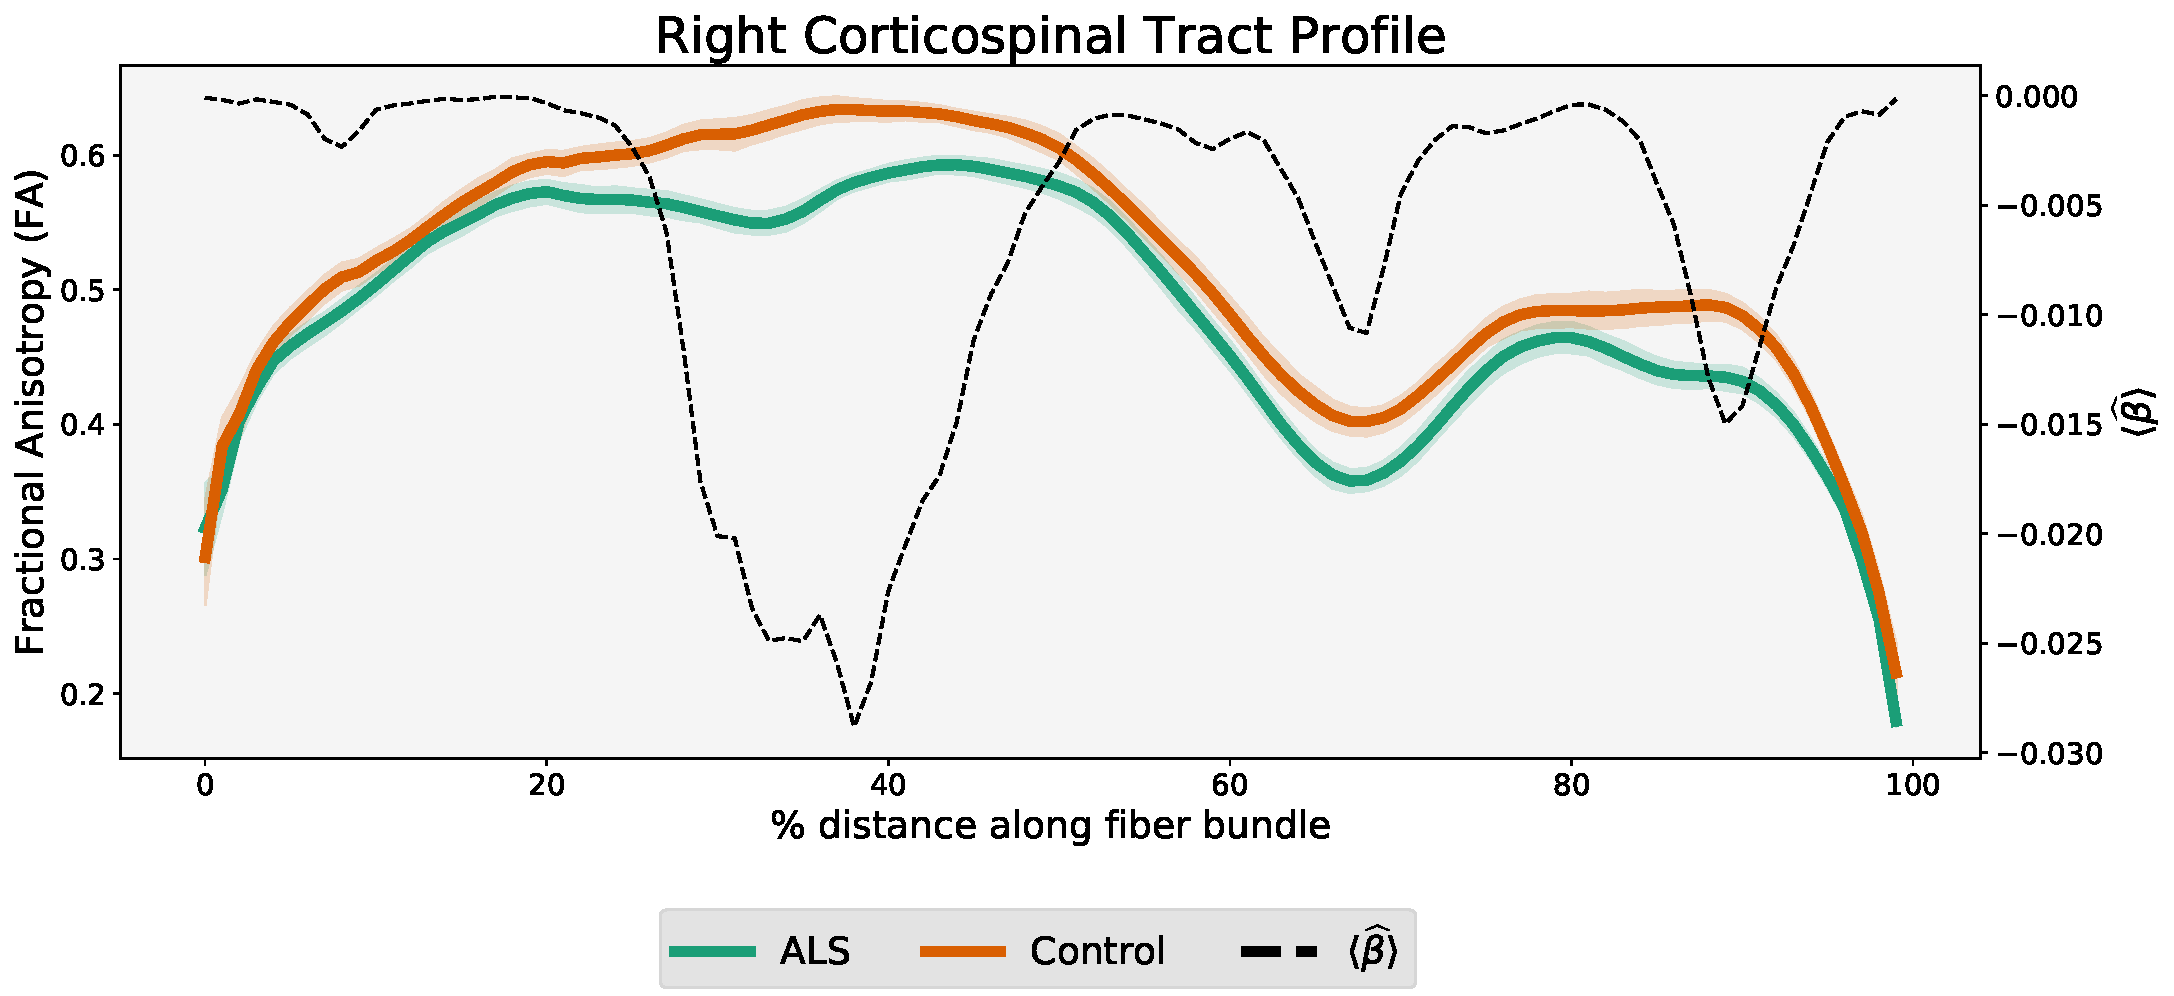
\includegraphics[width=0.95\textwidth]{classification_tract_profiles.pdf}
    \caption{{\bf Model coefficients mirror FA differences}. The places along the
       length of the CST  where $\hat{\beta}$ coefficients for FA
       (dashed line, right axis) have large negative values correspond to the
       locations of substantial differences between the ALS (green) and control
       (orange) FA (shaded area indicates standard error of the mean).}
    \label{fig:class-profiles}
\end{figure}

\begin{figure}[h]
    \centering
        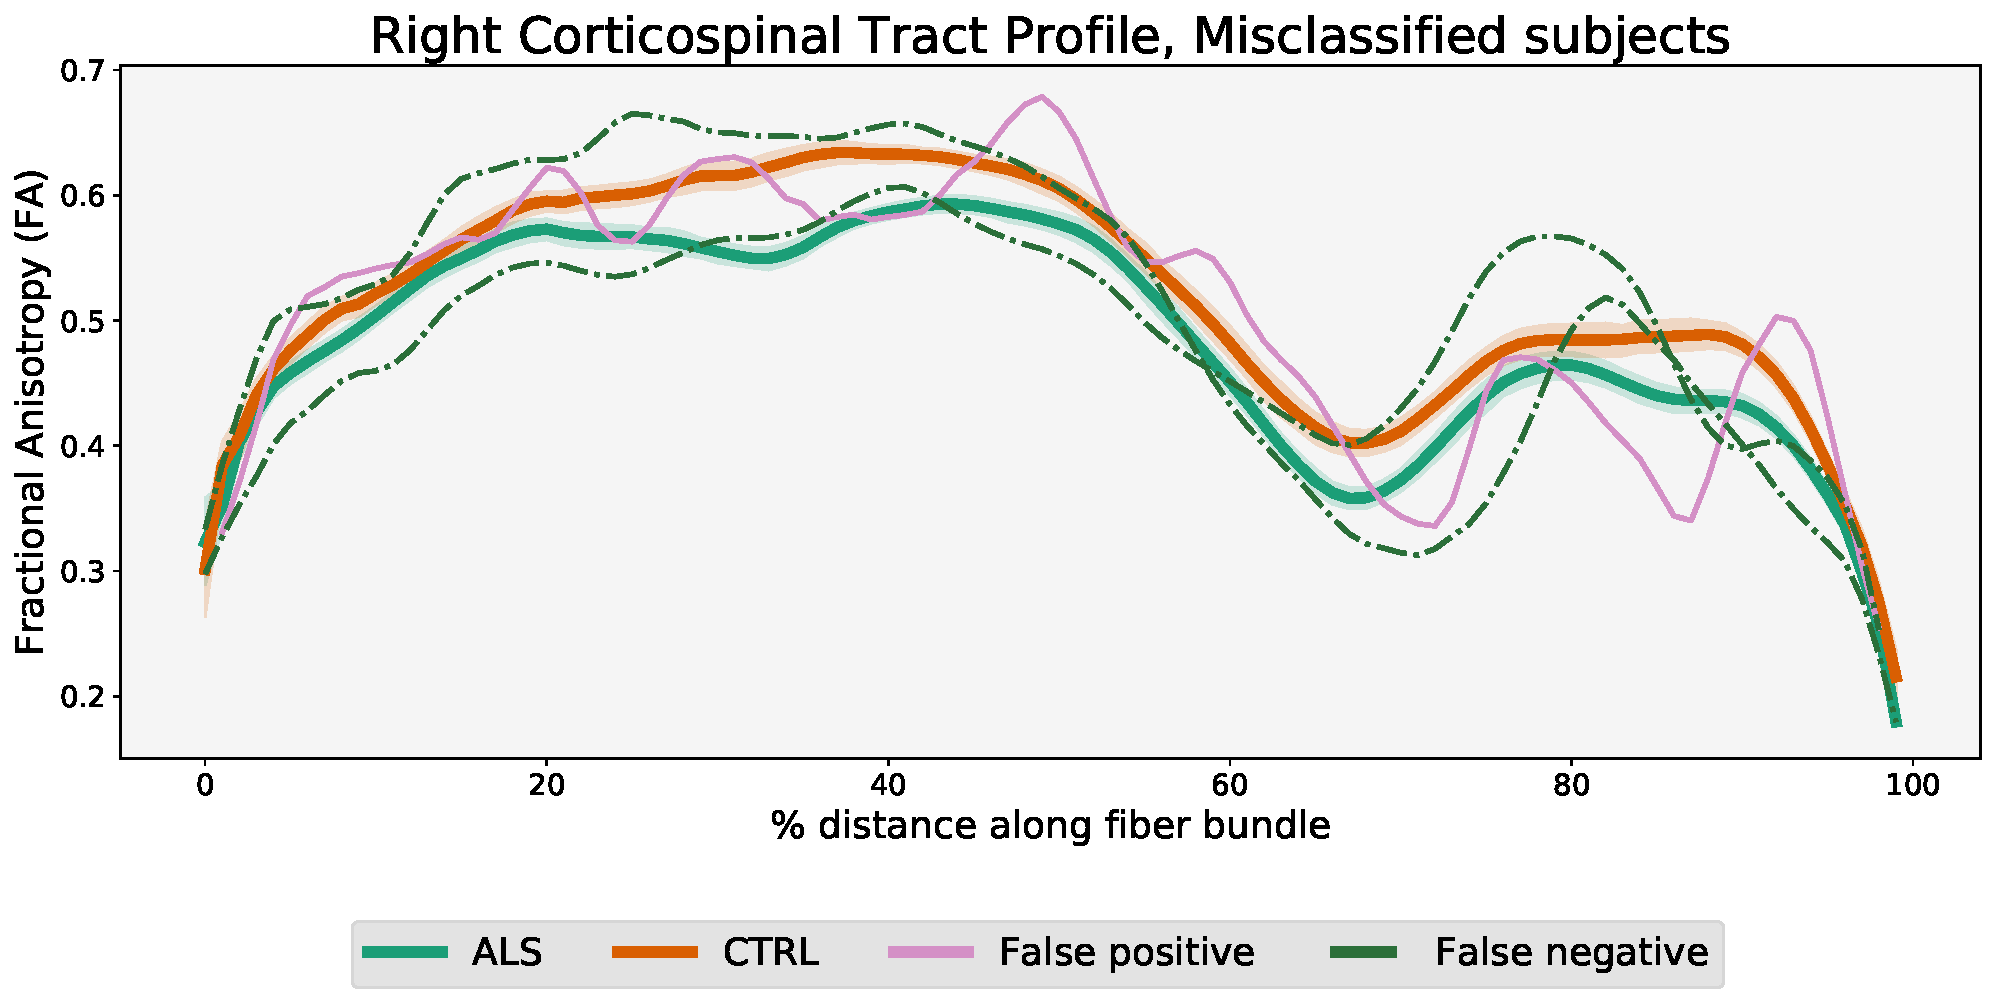
\includegraphics[width=0.95\textwidth]{classification_subjects_profiles.pdf}
    \caption{{\bf Model mis-classifications correspond to features identified by
       the model}. The FA in CST of individuals that are mis-classified by the
       model is compared the group FA (with shaded are indicating standard error
       of the mean). False negative classifications (individuals that have ALS,
       but are classified as patients) correspond to high FA either in one of
       the two regions of large $||\hat{\beta}||$ in
       Figure \ref{fig:class-profiles}. The false positive classification has
       an FA profile that oscillates between the two group means.
   }
    \label{fig:class-errors}
\end{figure}

\subsection*{SGL accurately predicts age from tractometry data in a regression setting}

To test the performance of SGL with tractometry data in a continuous regression
task, we focus here on the prediction of biological age based on tractometry
data. Prediction of ``brain age'' is a commonly undertaken task. This is both
because it operates on a natural scale, with meaningful and easily understood
units, as well as because predictions of brain age, and deviations from accurate
prediction are diagnostic of overall brain health (for a recent review, see
\cite{Cole2019-rz}). The WH dataset used here contains data from 76 healthy
subjects, ranging between 6 years and 50 years of age
\cite{yeatman2014lifespan}. In this case, biological age was used as the
predicted variable ($y$ in Eq~\eqref{eq:lm}). SGL was fit to
tractometry-extracted features: FA and MD in 20 major brain tracts, with each
tract divided into 100 nodes. To evaluate the fit of the model, we used a nested
cross-validation procedure. In this procedure, batches of subjects are held out.
For each batch (or fold), the model is fully fit without this data. Then, once
the parameters are fixed, the model is inverted to predict the ages of held out
subjects based on the linear coeffiecients and the static non-linearity. This
scheme automatically finds the right level of regularization (i.e., sparseness)
and fits the coefficients to the ill-posed linear model, while guarding against
overfitting. SGL accurately predicts the age of the subjects in this procedure,
with a mean absolute error of 3.6 years (Figure \ref{fig:regress-results}, left
panel). This is lower than the results of a recent study that predicted age in a
large sample, based on diffusion MRI features \cite{Richard2018-ux}.
Nevertheless, older subjects have higher residual variance, reflecting the
automatically-chosen log-transformation and implying that brain age becomes more
difficult to predict as we age chronologically (\ref{fig:regress-results}, right
panel). The model weights are distributed over many different tracts and dMRI
tissue properties (Figure \ref{fig:regress-beta} left). This demonstrates that
SGL is not coerced to produce overly sparse results when a more accurate model
requires a dense selection of features. Furthermore, looking closer at a
selection of tracts where high coefficients are found demonstrates that
diffusion properties (FA, in this case) are different in different age groups in
parts of the tracts where these higher coefficients are found (Figure
\ref{fig:regress-beta} right).


\begin{figure}[h]
    \centering
    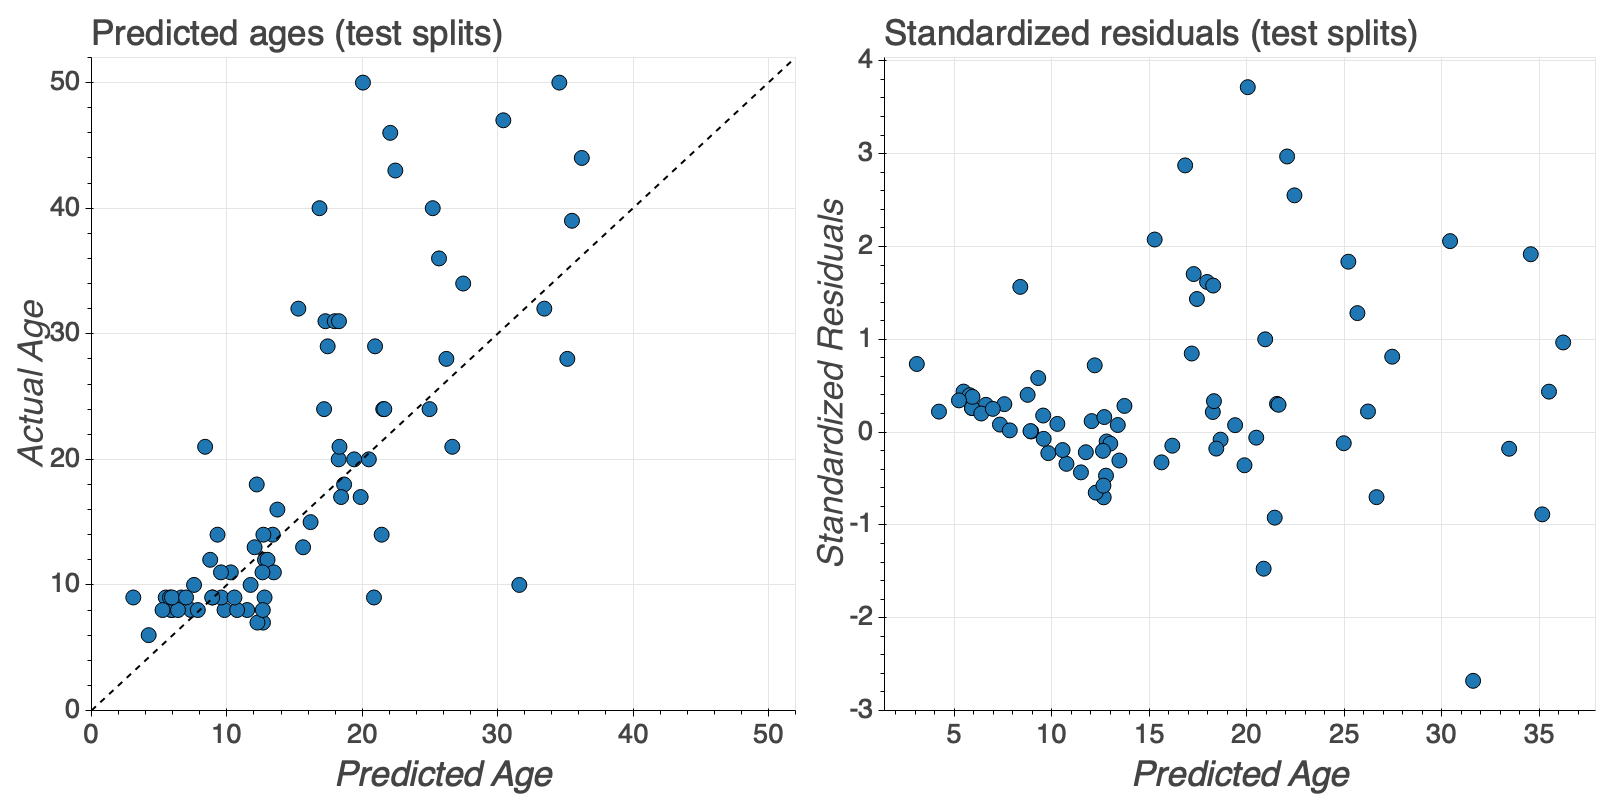
\includegraphics[width=0.8\textwidth]{regression_residuals.png}
    \caption{{\bf Predicting age with tractometry and SGL.} Left: The predicted
    age of each individual (on the abscissa) and true age (on the ordinate),
    from the test splits (i.e., when each subject's data was held out in fitting
    the model); an accurate prediction falls close to the $y=x$ line (dashed).
    The mean absolute error in this case is 3.6 years and, the coefficient of
    determination $R^2=0.3$. Right: Standardized residuals (on the abscissa) as
    a function of the true age (on the ordinate). Predictions are generally more
    accurate for younger individuals.}
    \label{fig:regress-results}
\end{figure}

\begin{figure}[h]
    \centering
    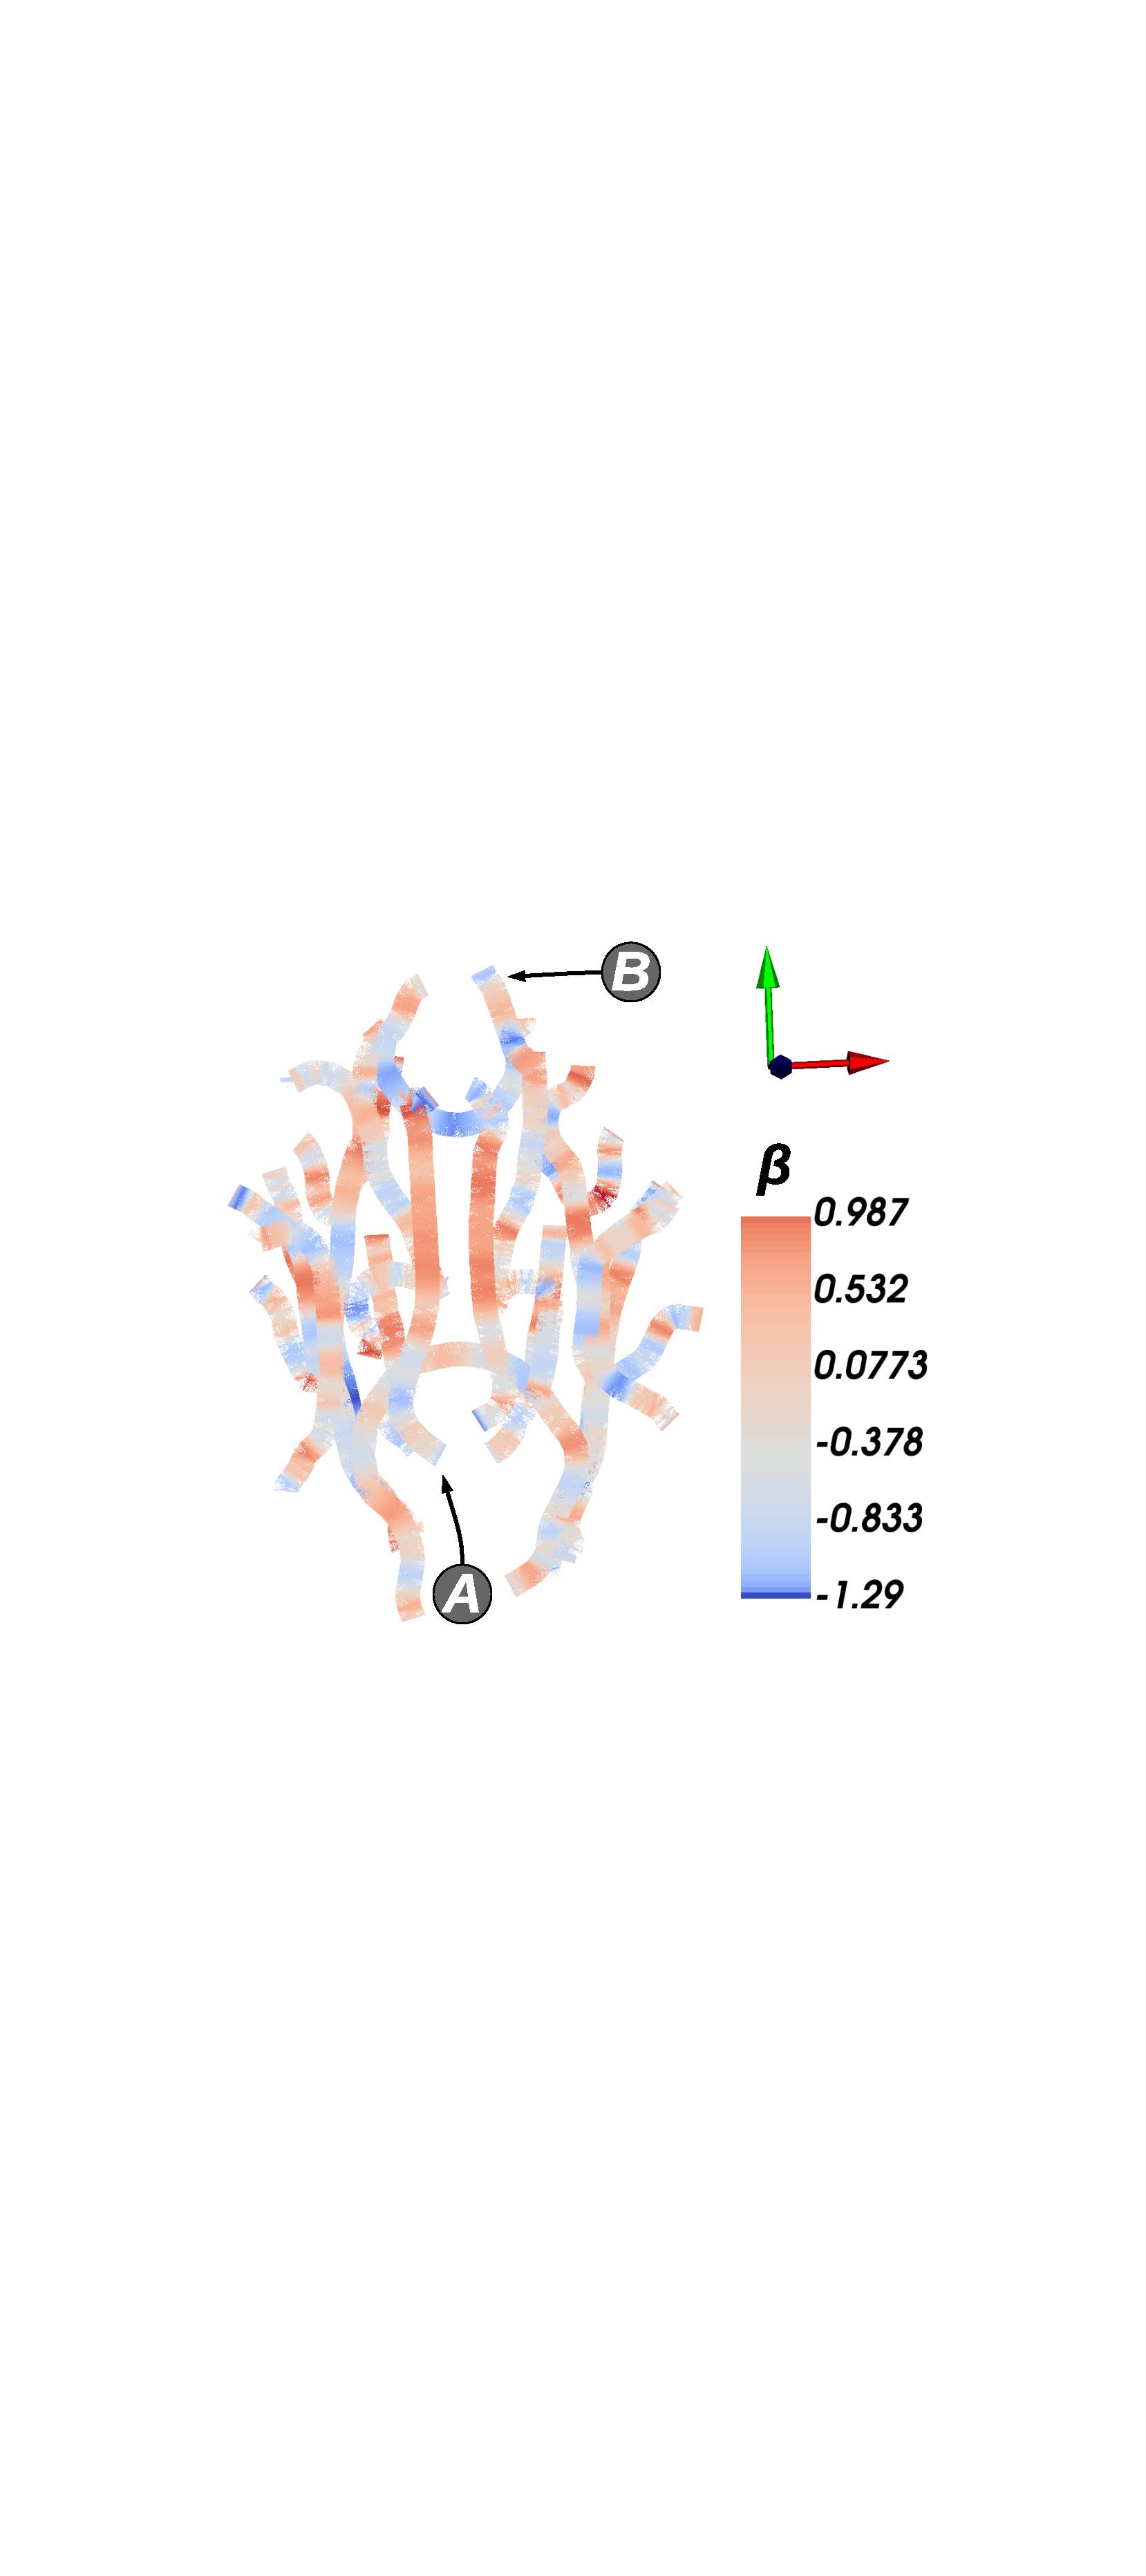
\includegraphics[width=0.3\textwidth]{regression_beta_annotated.pdf}
    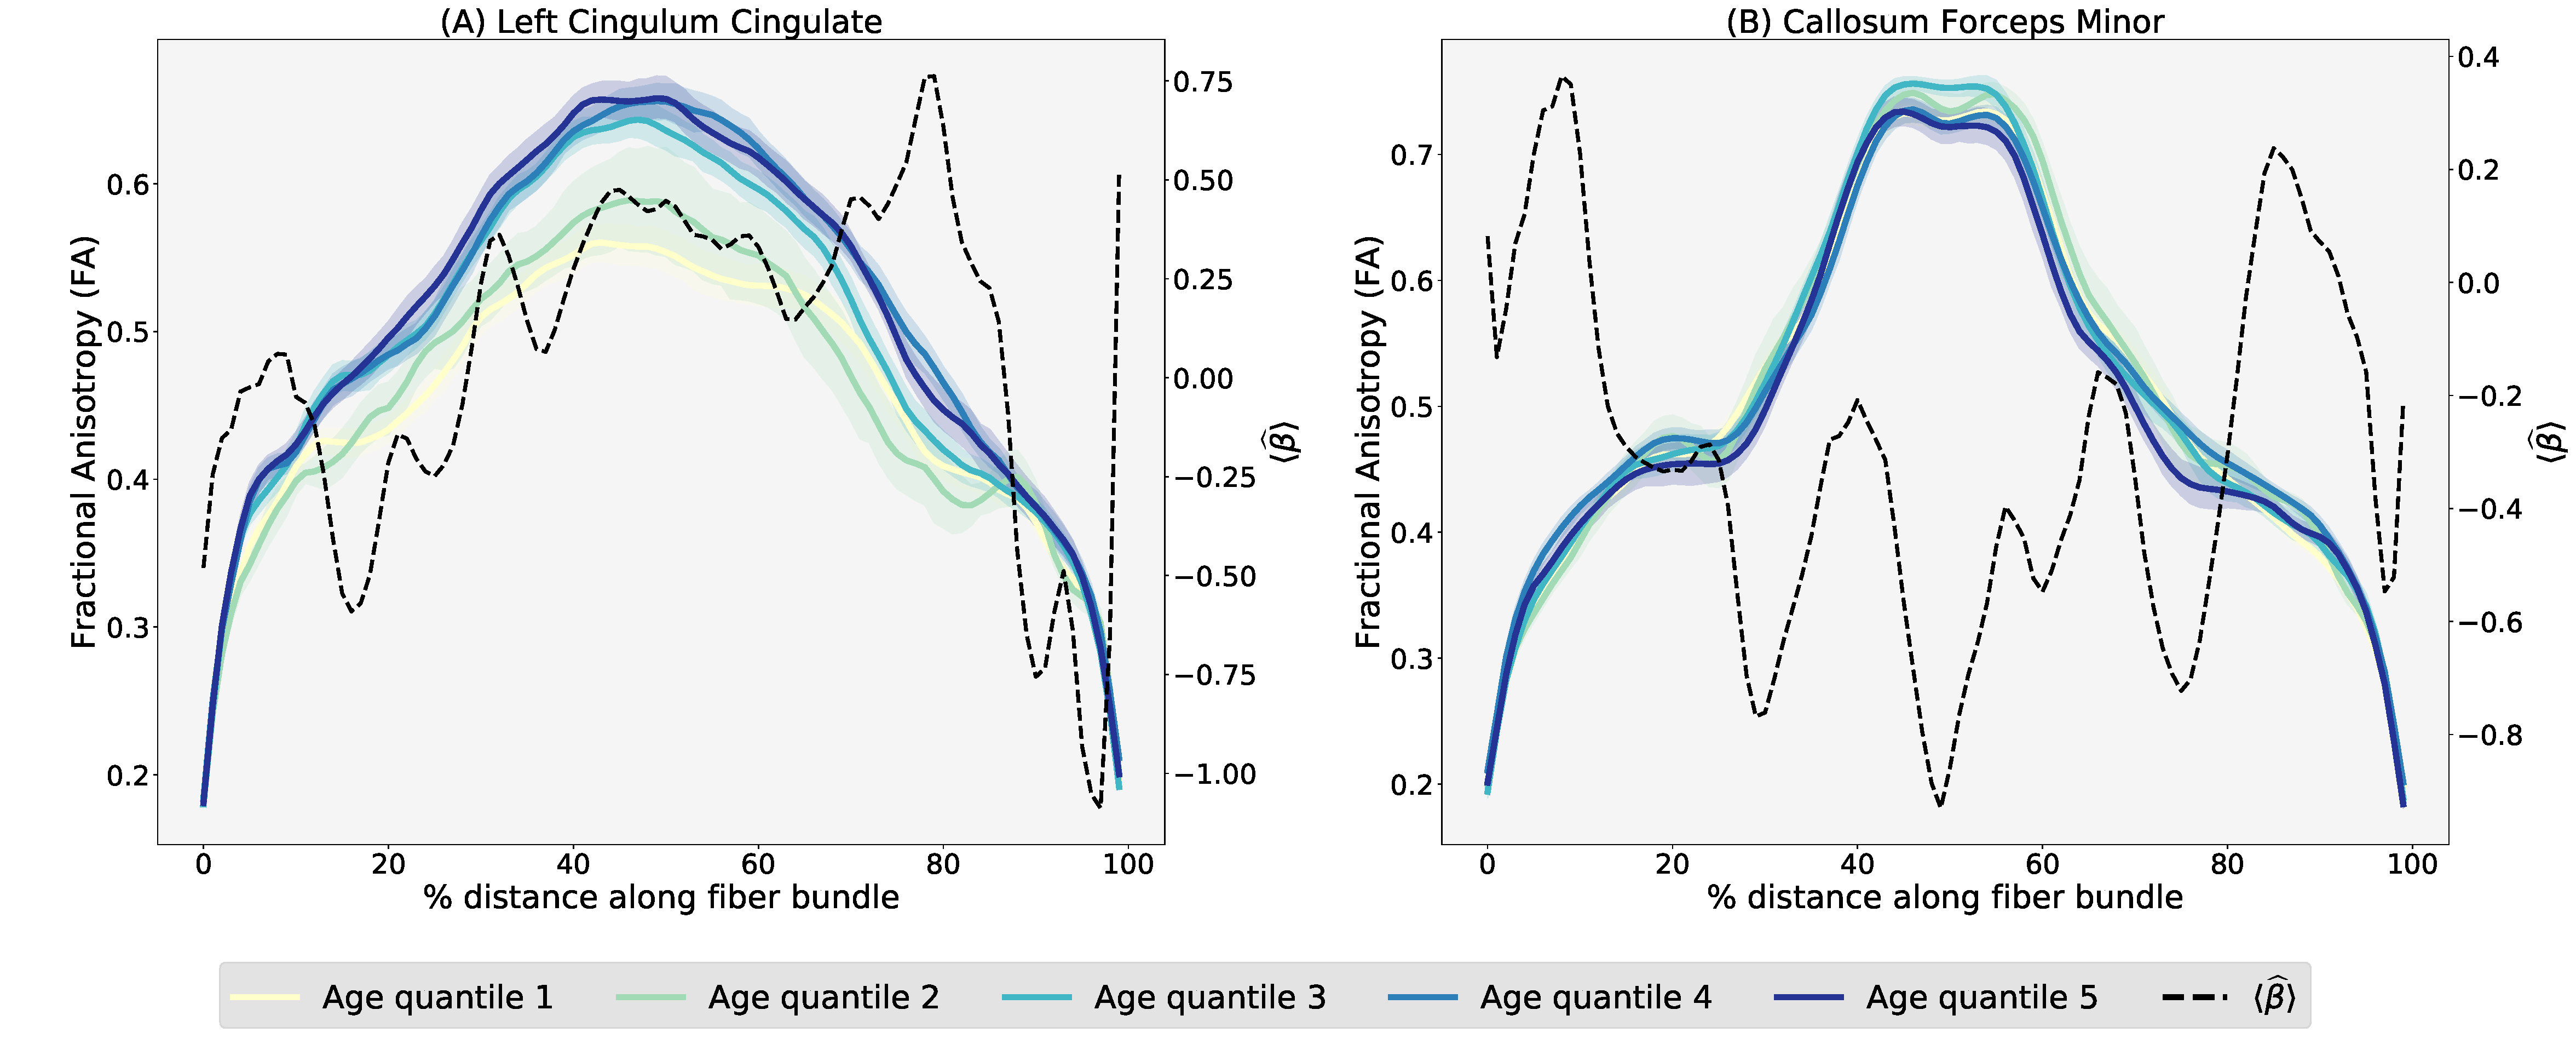
\includegraphics[width=0.67\textwidth]{regression_tract_profiles.pdf}
    \caption{{\bf Feature importance for predicting age from tractometry.} Left:
    A skeletonized display of the main brain tracts analyzed, with anterior
    facing up, and right hemisphere on the right. The $\hat{\beta}$ coefficients
    displayed in blue (negative) to red (positive) are for measurements of FA
    along the length of the tracts. The left cingulum cingulate (A) and forceps
    minor (B) are highlighted. Right: the FA (in shades of blue and green) and
    the $beta$ coefficients (dashed) in (A) left cingulum and (B) forceps
    minor.}
    \label{fig:regress-beta}
\end{figure}


\section*{Conclusion}

We present here a novel method for analysis of dMRI tractometry data. This
method relies on the Sparse Group Lasso \cite{simon2013sparse} to provide both
accurate prediction of the phenotypic properties of individual subjects based on
their dMRI data, but also provides interpretable results by identifying the
features that are important across subjects to make these predictions. The
method is broadly applicable: it performs well in predicting both continuous
variables, such as biological age, as well as discrete variable, such as whether
a person is a patient or a healthy control. In both of these cases, SGL
out-performs previous algorithms that have been developed for these tasks
\cite{sarica2017corticospinal, Richard2018-ux}. The nested cross-validation
approach used to fit the model and make both predictioons and inferences from it
guards against overfitting and tunes the degree of sparseness required by the
algorithm, such that both phenomena that are locally focused in a particular
anatomical location and a particular property of diffusion (e.g., FA in the
CST), as well as widely distributed phenomena can be accurately captured.

Specifically, we demonstrated that the algorithm correctly detects the fact that
ALS, which is a disease of lower motor neurons, is localized to the
cortico-spinal tract. This recapitulates the results of previous analysis of
these same data, using a targetted ROI-based approach
\cite{sarica2017corticospinal}. In contrast, in analysis of biological age, the
coefficients identified by the algorithm are very widely distributed in many
parts of the white matter, mirroring previous results with this dataset that
show a large and continuous distribution of life-span changes in white matter
properties \cite{yeatman2014lifespan}.

Taken together, these results demonstrate the promise of the group-regularized
regression approach. Even at the scale of dozens of subjects, the results
provided by SGL are both accurate and interpretable. Thus, this multivariate
analysis approach both (a) achieves high cross-validated accuracy for precision
medicine applications of dMRI data and (b) identifies relevant features of brain
anatomy that can further our neuroscientific understanding of clinical
disorders.

Meanwhile, neuroscience has entered an era in which consortium efforts are
putting together large datasets of high-quality dMRI data to address a variety
of scientific questions \cite{jernigan2016ping, jernigan2018abcd,
alexander2017open, Miller2016-hw, VanEssen2012}. The volume and complexity of
these data pose a substantial challenge. Dimensionality reduction with
tractometry, followed by analysis with the approach we present here promises to
capitalize on the wealth of data and on the co-measurement of interesting and
important phenotypical data about brain health and about the participants'
cognitive abilities. We also expect the group-regularized approach to improve
with larger datasets.

SGL has many other potential applications in neuroscience, because of the
hierarchical and grouped nature of many of the data -- that are collected in
multiple sample points within anatomically-defined areas. For example, this
method may be useful to understand the relationship between fMRI recordings and
behavior, where activity in each voxel may co-vary with voxels within the same
anatomical region and form features and groups of features. Similarly,
large-scale multi-electrode recordings of neural activity in awake behaving
animals are becoming increasingly feasible \cite{steinmetz2018distributed,
Jun2017-gv} and these recordings can form features (neurons) and groups (neurons
within an anatomical region). More ambitiously perhaps, this approach may be
used to understand the role of correlations in so-called resting-state fMRI
time-series and behavior, where pairwise correlations between voxels in
different anatomical regions are features in the matrix and features may be
grouped by pairs of anatomical regions. Given the large number of voxels in the
surface of the gray matter, and given that correlations increase the number of
features by a factor of $n^2$ this would be a challenging problem to solve using
SGL.

The results we present here also motivate extensions of the method using more
sophisticated cost functions. For example, the fused sparse group lasso (FSGL)
\cite{zhou2012} extends SGL to enforce additional spatial structure: smoothness
in the variation of diffusion metrics along the tracts. As brain measurements
include additional structure (for example, bilateral symmetry), future work
could also incorporate overlapping group membership for each entry in the tract
profiles \ariel{citation needed}. For example, a measurement could come from the
corpus callosum, but also from the right hemipshere. This would also require
extending the cost function used here to incorporate these constraints.

The method is packaged as open-source software called AFQ-Insight that is openly
available, and this also where extensions of the method will be developed. The
sofware integrates within a broader automated fiber quantification software
ecosystem: AFQ \cite{yeatman2012tract}, which extracts tractometry data from raw
and processed dMRI datasets, as well as AFQ-Browser, which visualizes
tractometry data and facilitates sharing of the results of dMRI studies
\cite{yeatman2018browser}. To facilitate reproducibility and ease use of the
software, the results presented in this paper are also provided in
\url{https://github.com/richford/afq-insight-paper} as a series of Jupyter
notebooks
\cite{kluyver2016jupyter}



\section{Acknowledgements}

Here are some amazing acknowledgements.


\bibliographystyle{abbrv}
\bibliography{paper}

\end{document}
